\section{Dashboard web (item 2b)}

\subsection{Função e telas}

A Dashboard é servida pelo receptor (\cod{run\_receiver.ps1}, módulo \cod{simulador/web/dashboard.py}, FastAPI + uvicorn) na porta 8081 e é atualizada a cada 1 s pelo WebSocket \cod{/ws}. O indicador ``OPC UA conectado'' no cabeçalho é verde quando a última notificação do Gateway tem menos de 10 s (\cod{opcua\_stale\_seconds}). A página principal tem três blocos:

\begin{itemize}
    \item \textbf{Postos da linha} - uma coluna por posto com status, Takt time, Cycle time (último ciclo), Disponibilidade, Desempenho, Qualidade e OEE. A cor da coluna segue o estado \cod{D01651}-\cod{D01662}: amarelo nos estados 0 e 1 (aguardando), verde piscando no 2 (processando) e verde constante no 3 (finalizou). Com um Andon ativo, a coluna do posto fica vermelha e as demais cinza (``Linha parada'').
    \item \textbf{Plano e acompanhamento} - meta de produção e tempo disponível (editáveis em \textbf{Editar plano do turno}), tempo decorrido, tempo real de produção, produção estimada, produção atual (contador \cod{D16052}) e defeitos.
    \item \textbf{OEE da linha e Parada da linha} - os três fatores, o OEE consolidado e os minutos parados por categoria de Andon.
\end{itemize}

A página \cod{/graficos} mostra o último ciclo (ou o Takt) de cada posto em barras, e o botão \textbf{IT Digital E07} abre a instrução de trabalho (seção 7). \textbf{Importar base}, \textbf{Start} e \textbf{Limpar base} acionam o CLP pelo caminho da Tabela \ref{tab:comandos}; o Start só é habilitado com a base conferida, os 12 postos no estado 0 e nenhum Andon ativo.

\subsection{Indicadores calculados}

Os cálculos estão em \cod{services/analytics.py} (revisão \cod{2026-11-20.01}, publicada em \cod{/api/version}). O período de medição começa no Start confirmado pelo CLP (ou no último reset) e termina no instante atual. Sendo $T$ o tempo decorrido, $S$ o tempo parado, $M$ a meta do turno, $T_d$ o tempo disponível, $B$ as peças boas (contador do P12) e $D$ os defeitos:

\begin{align*}
\text{Produção esperada} &= M \cdot \frac{T}{60\,T_d} \\
\text{Produção estimada} &= \lfloor \text{Produção esperada} \rfloor \\
\text{Disponibilidade} &= 100 \cdot \frac{T - S}{T} \\
\text{Desempenho} &= 100 \cdot \frac{B}{\text{Produção estimada}} \\
\text{Qualidade} &= 100 \cdot \frac{B}{B + D} \\
\text{OEE} &= \frac{\text{Disponibilidade} \cdot \text{Desempenho} \cdot \text{Qualidade}}{10^4}
\end{align*}

O tempo parado $S$ é a \textbf{união} dos intervalos de todos os Andons (intervalos sobrepostos não são somados duas vezes); os minutos por categoria são calculados separadamente e a sobreposição é informada à parte. Um Andon de Qualidade ligado registra um defeito no posto. O Desempenho só é exibido quando há ao menos uma peça boa e uma peça estimada.

\subsection{Evidência: execução com o Gateway real e o CLP emulado}

A demonstração da seção \ref{sec:emulado} foi acompanhada pela Dashboard. O plano foi definido por \cod{PUT /api/process/production-plan} com meta de 90 peças em 60 min (Takt de 40 s) e a base \cod{base\_demo.csv} foi importada (P07 com ciclo de 36 s, demais postos entre 6 e 12 s). As Figuras \ref{fig:dash1} a \ref{fig:dash5} são capturas da página real, sem edição além do corte da área vazia.

\begin{figure}[H]
    \centering
    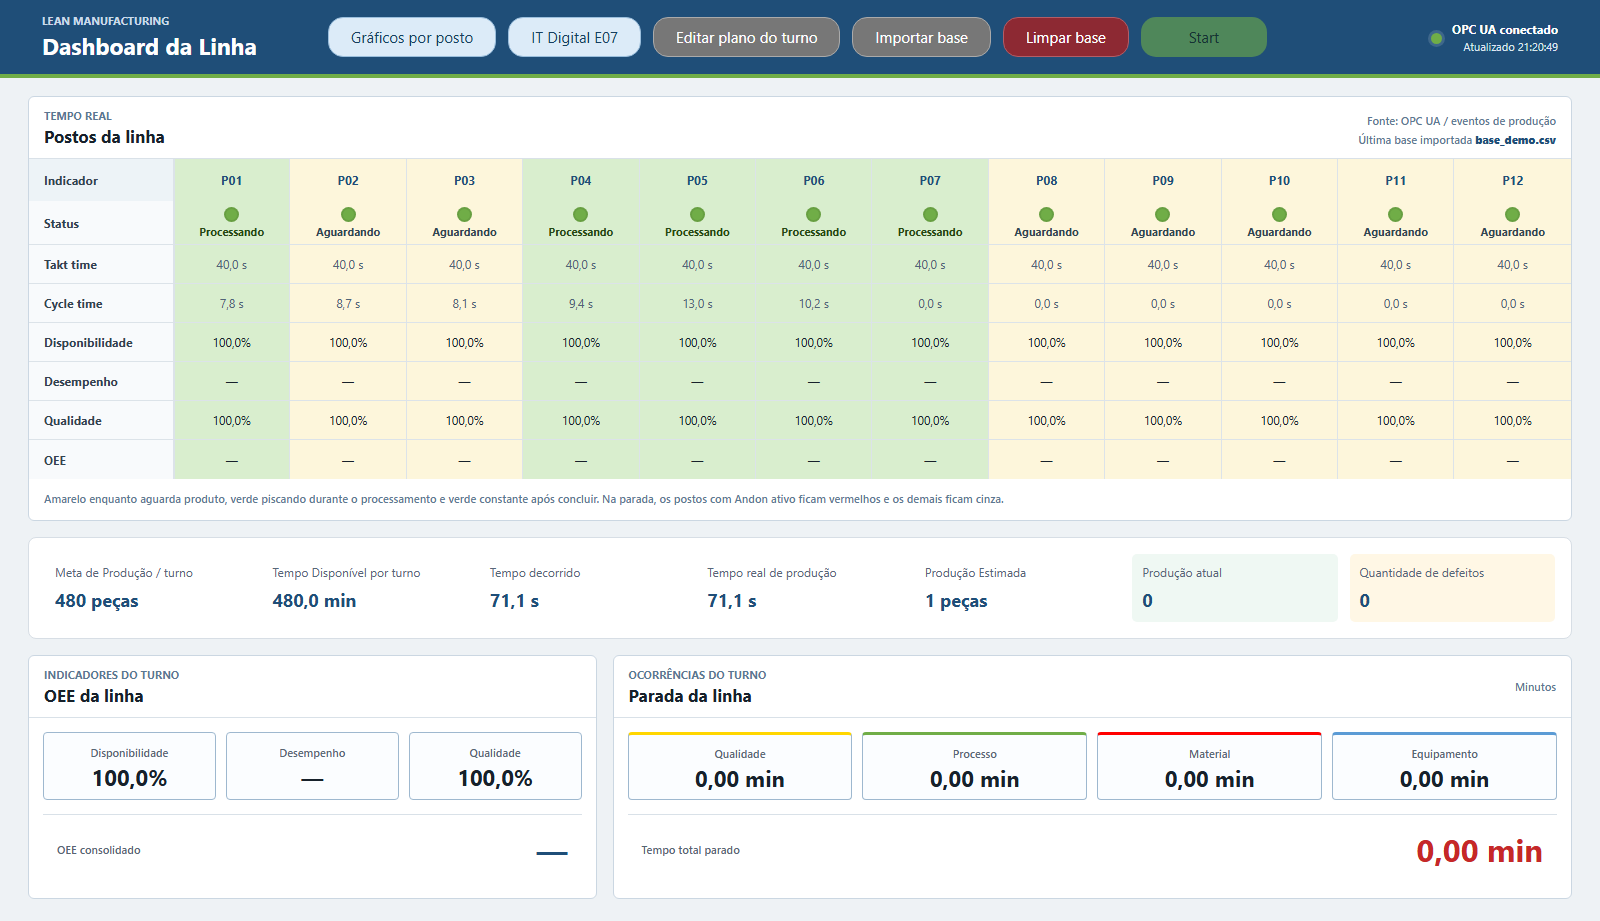
\includegraphics[width=1.00\textwidth]{Imagens/dash_06_p07_processando.png}
    \caption{Linha em operação: P01 e P04 a P07 processando (verde), demais aguardando (amarelo); nenhuma parada. (arquivo: Imagens/dash\_06\_p07\_processando.png)}
    \label{fig:dash1}
\end{figure}

\begin{figure}[H]
    \centering
    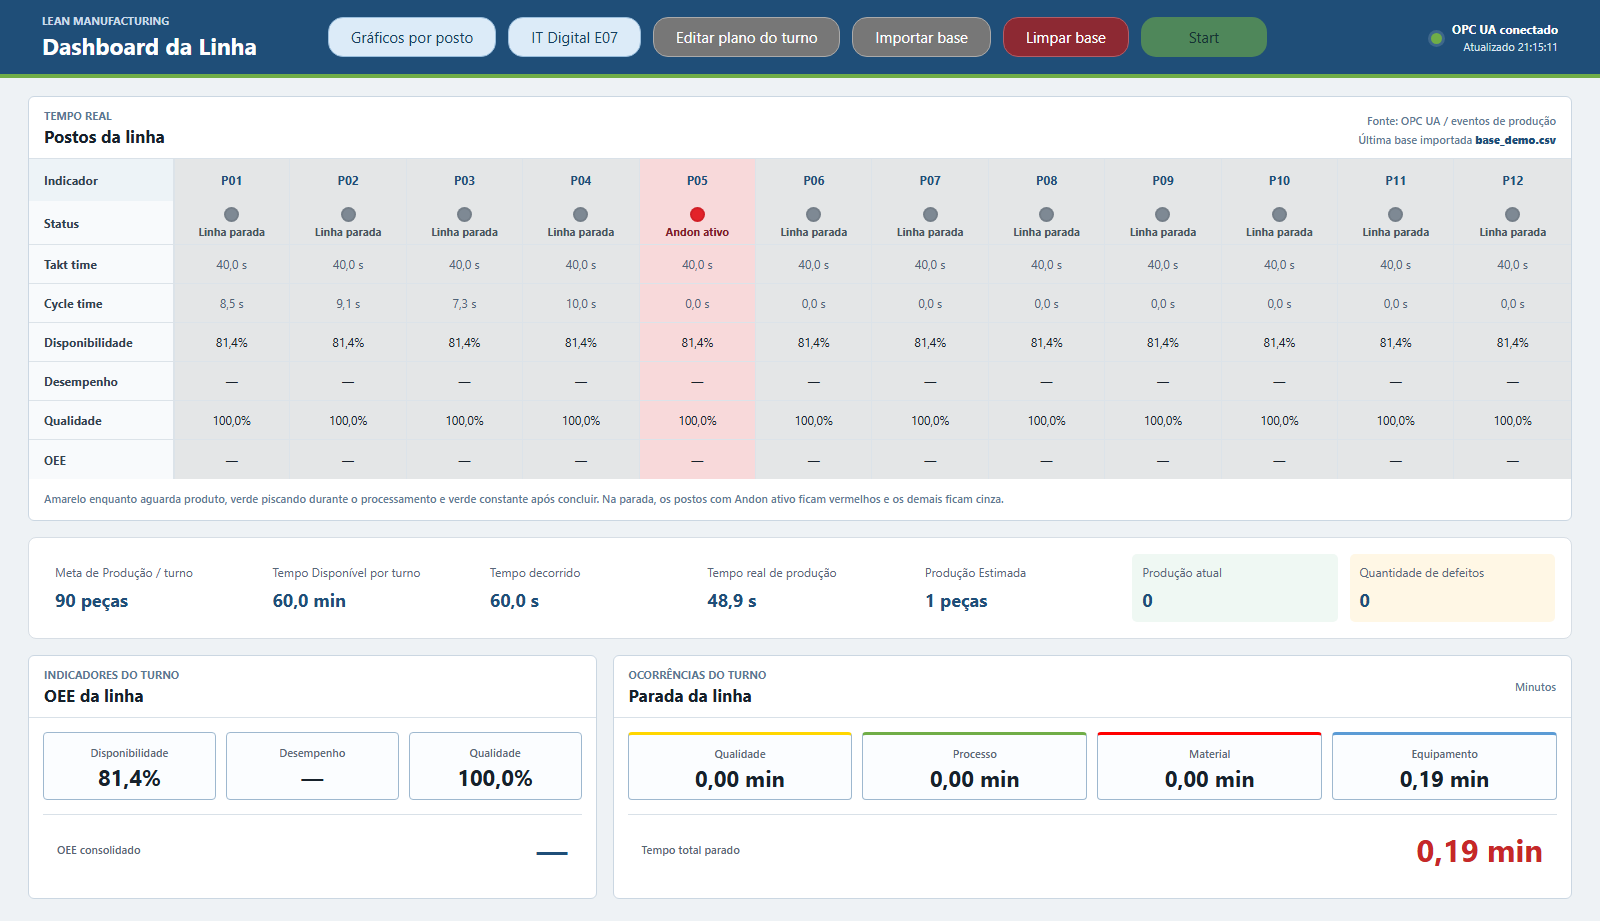
\includegraphics[width=1.00\textwidth]{Imagens/dash_02_andon_p05.png}
    \caption{Andon de Equipamento no P05, 50 s após o Start: coluna P05 vermelha, demais em ``Linha parada''; disponibilidade caindo (81,4 \%) e 0,19 min de parada por Equipamento. (arquivo: Imagens/dash\_02\_andon\_p05.png)}
    \label{fig:dash2}
\end{figure}

\begin{figure}[H]
    \centering
    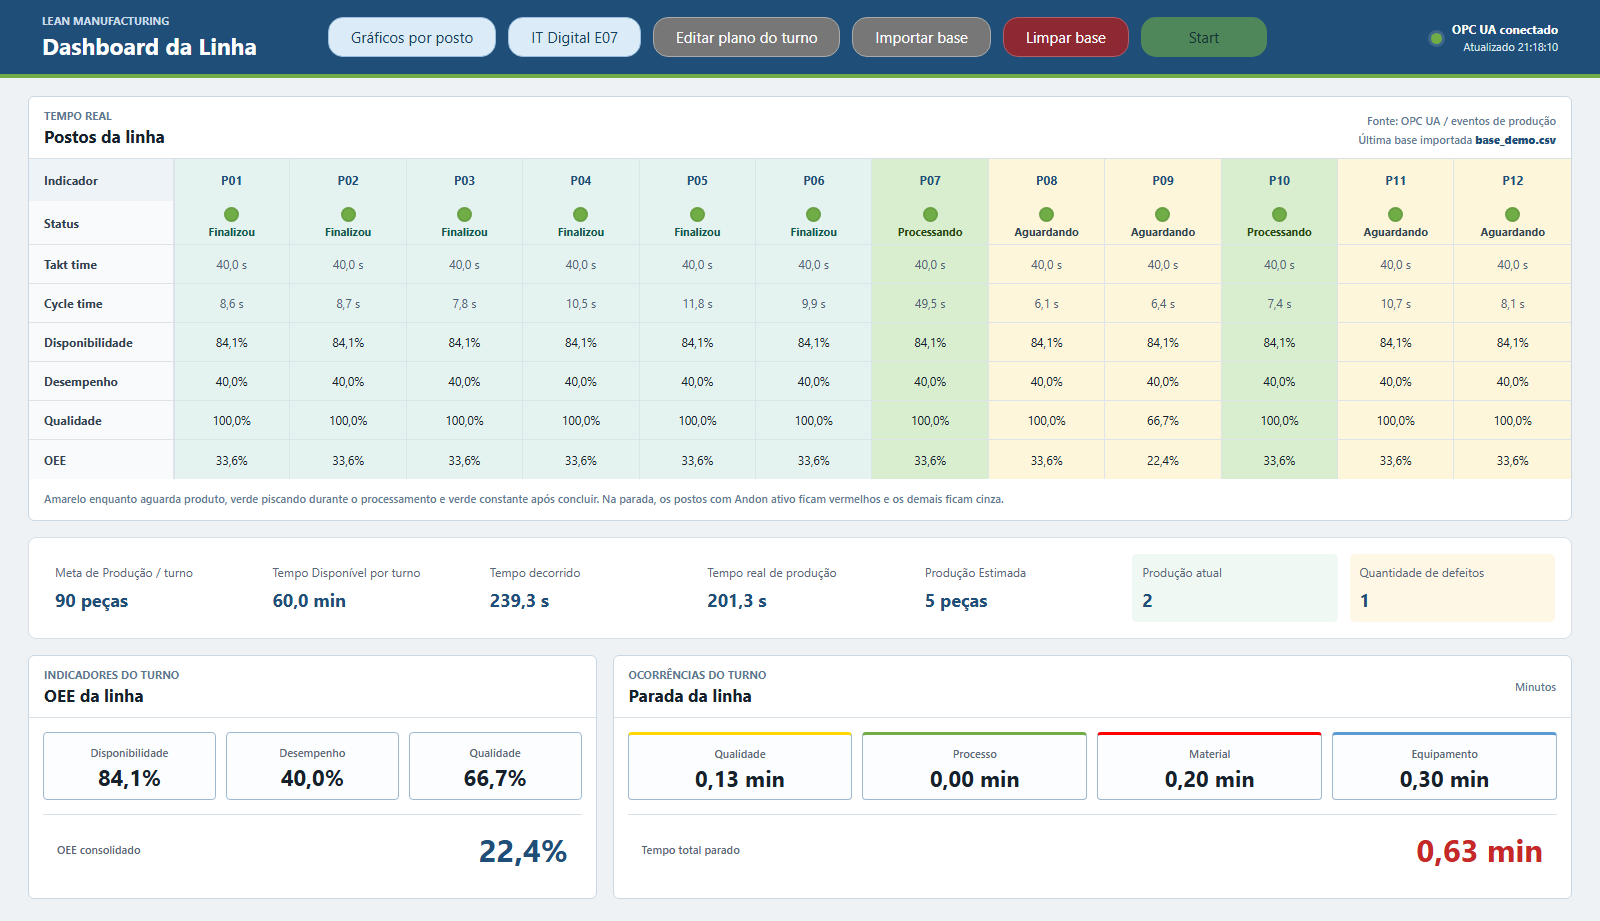
\includegraphics[width=1.00\textwidth]{Imagens/dash_03_final.png}
    \caption{Situação após 239,3 s: 2 peças produzidas, 1 defeito (Andon de Qualidade no P09), 0,63 min parados (Qualidade 0,13, Material 0,20 e Equipamento 0,30) e OEE de 22,4 \%. (arquivo: Imagens/dash\_03\_final.png)}
    \label{fig:dash3}
\end{figure}

\textbf{Conferência numérica da Figura \ref{fig:dash3}.} Com $T = 239{,}3$ s e $S = 38{,}0$ s (0,13 + 0,20 + 0,30 = 0,63 min, sem sobreposição), a Disponibilidade é $100 \cdot (239{,}3 - 38{,}0) / 239{,}3 = 84{,}1$ \%. A produção esperada é $90 \cdot 239{,}3 / 3600 = 5{,}98$, logo a estimada é 5 peças e o Desempenho é $100 \cdot 2/5 = 40{,}0$ \%. A Qualidade é $100 \cdot 2/(2+1) = 66{,}7$ \% na linha e no P09; nos demais postos, sem defeito, é 100 \%. O OEE é $84{,}1 \times 40{,}0 \times 66{,}7 / 10^4 = 22{,}4$ \% na linha e no P09 e $84{,}1 \times 40{,}0 \times 100 / 10^4 = 33{,}6$ \% nos demais postos - exatamente os valores exibidos.

\begin{figure}[H]
    \centering
    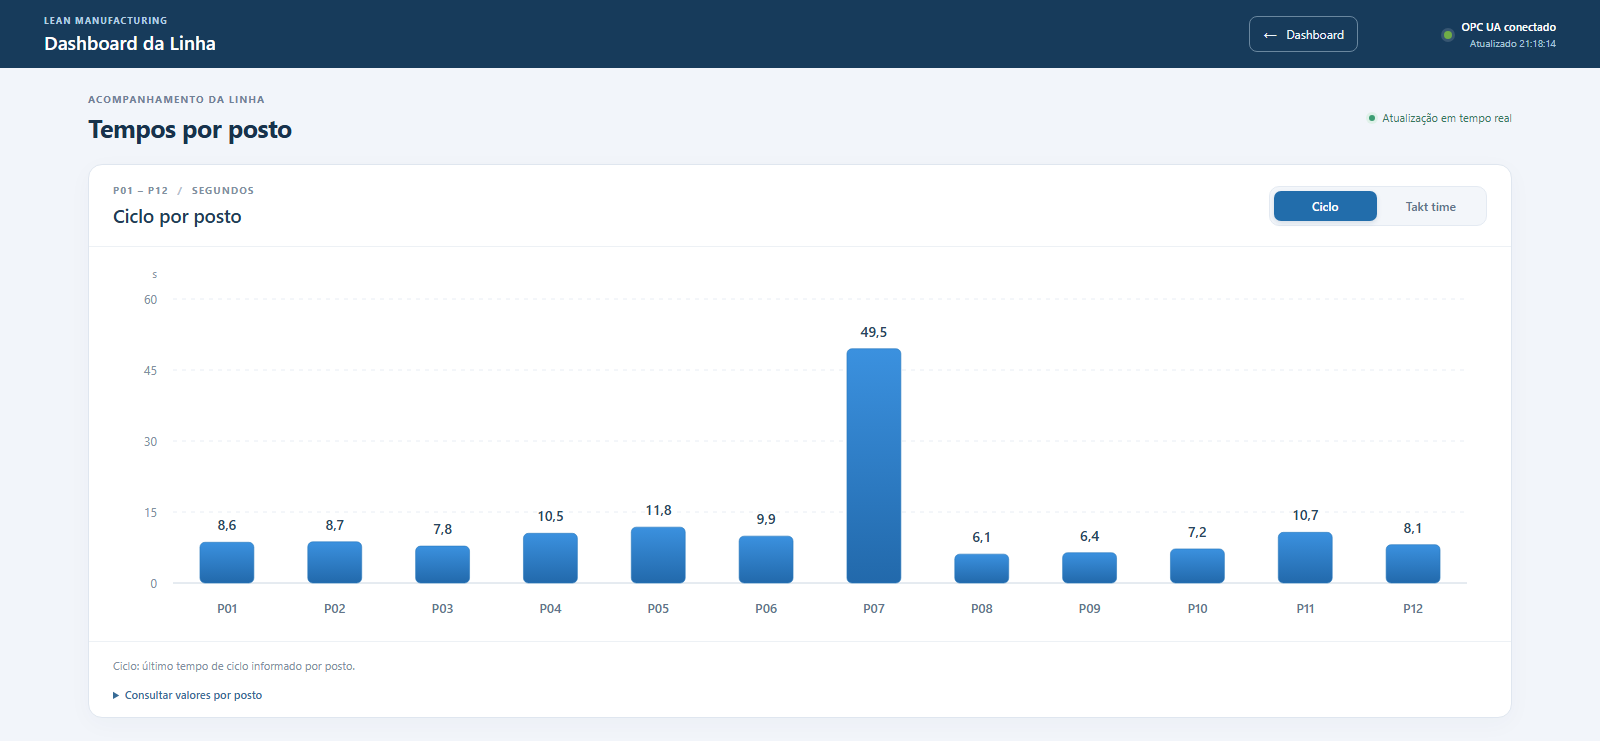
\includegraphics[width=1.00\textwidth]{Imagens/dash_04_graficos.png}
    \caption{Página \cod{/graficos}: último ciclo por posto. O P07 (49,5 s, contra Takt de 40 s) é o gargalo; o ciclo medido inclui o tempo em que o posto ficou parado pelos Andons. (arquivo: Imagens/dash\_04\_graficos.png)}
    \label{fig:dash4}
\end{figure}

\begin{figure}[H]
    \centering
    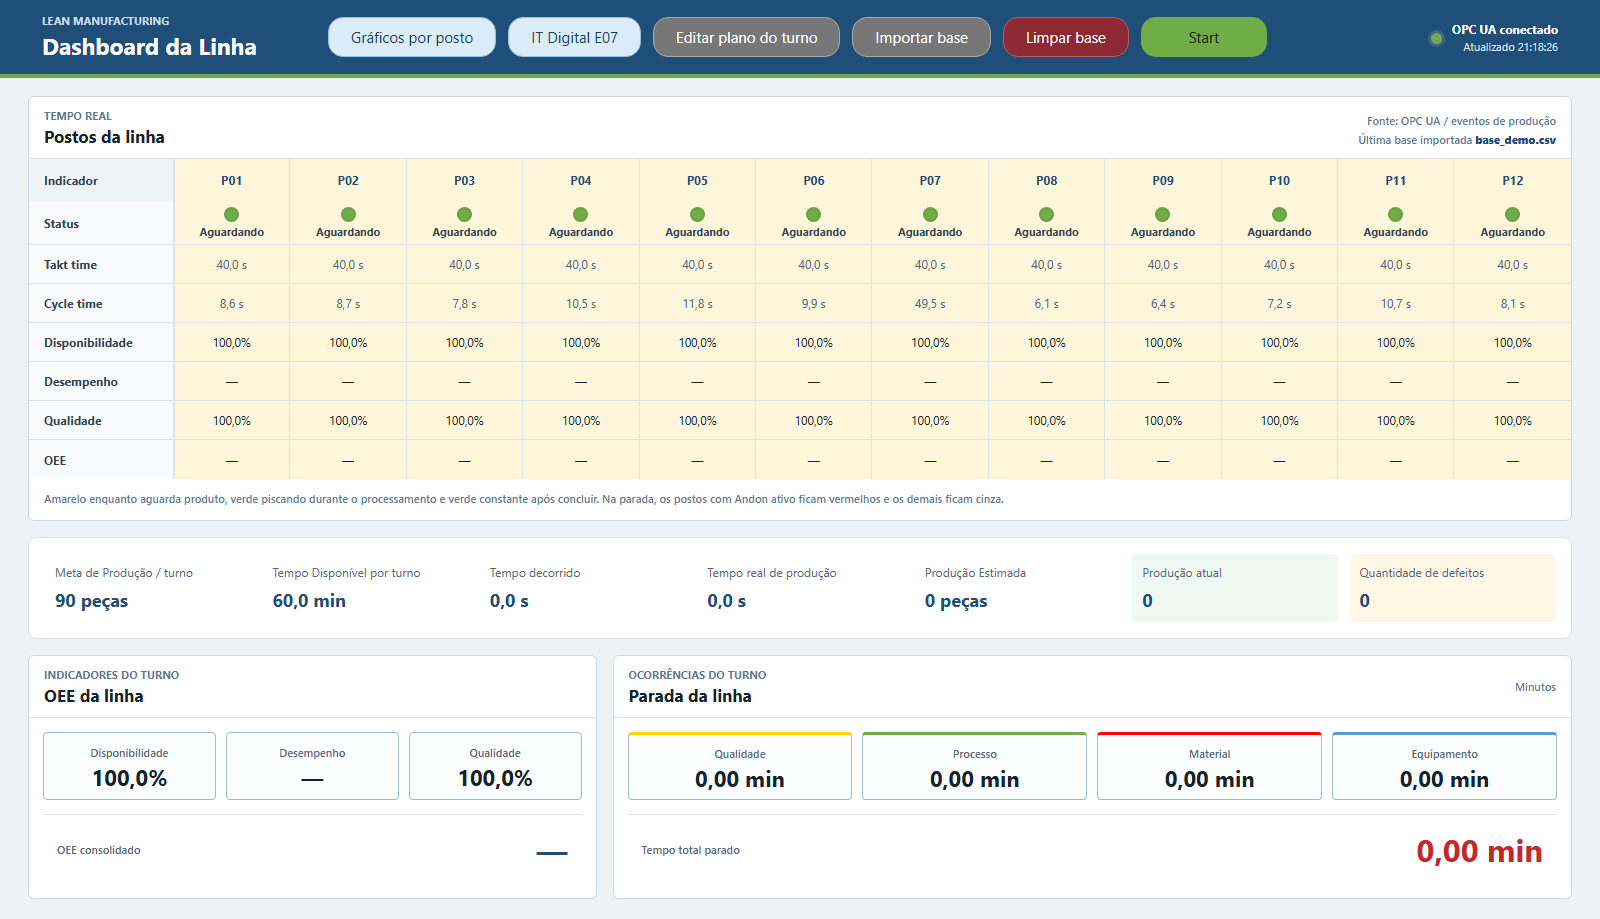
\includegraphics[width=1.00\textwidth]{Imagens/dash_05_apos_limpar.png}
    \caption{Após \textbf{Limpar base} (\cod{P10003} e \cod{D16052 = 0} conferidos): 12 postos aguardando, produção, defeitos e paradas do dia zerados e Start novamente habilitado. (arquivo: Imagens/dash\_05\_apos\_limpar.png)}
    \label{fig:dash5}
\end{figure}

A Figura \ref{fig:estados} reconstrói, a partir de 90 amostras de \cod{/api/snapshot}, os estados que a Dashboard recebeu para cada posto. Vê-se a primeira peça percorrer os postos em sequência, a fila que se forma antes do P07 (P01 a P06 em ``concluído'', aguardando a liberação do posto seguinte) e as paradas provocadas pelos Andons. A Figura \ref{fig:oee} mostra a produção atual acompanhando a estimada e a queda da disponibilidade a cada parada.

\begin{figure}[H]
    \centering
    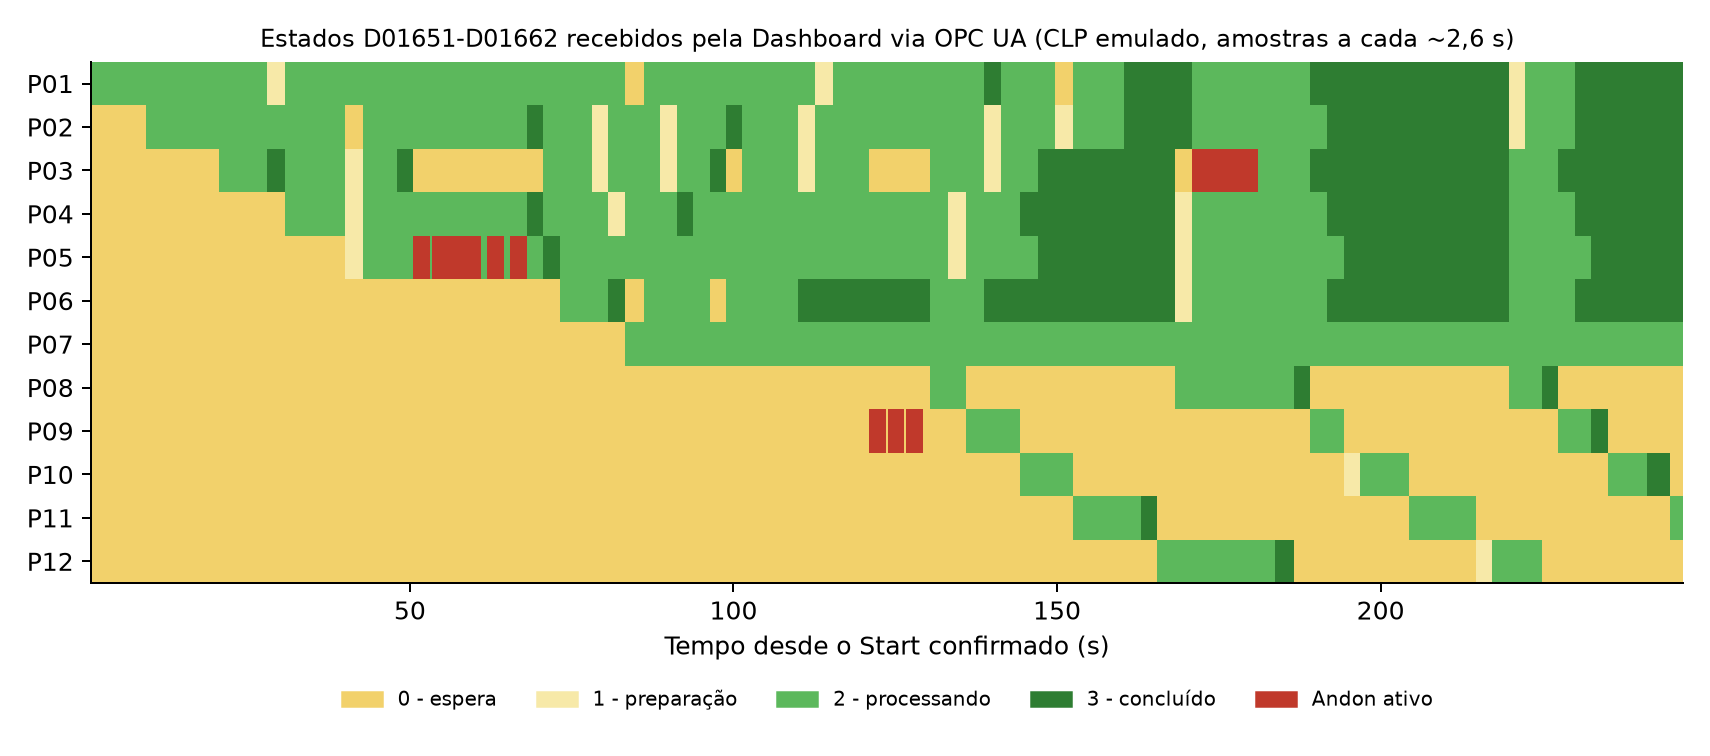
\includegraphics[width=1.00\textwidth]{Imagens/demo_estados_postos.png}
    \caption{Estados dos 12 postos recebidos pela Dashboard durante a demonstração (CLP emulado). (arquivo: Imagens/demo\_estados\_postos.png)}
    \label{fig:estados}
\end{figure}

\begin{figure}[H]
    \centering
    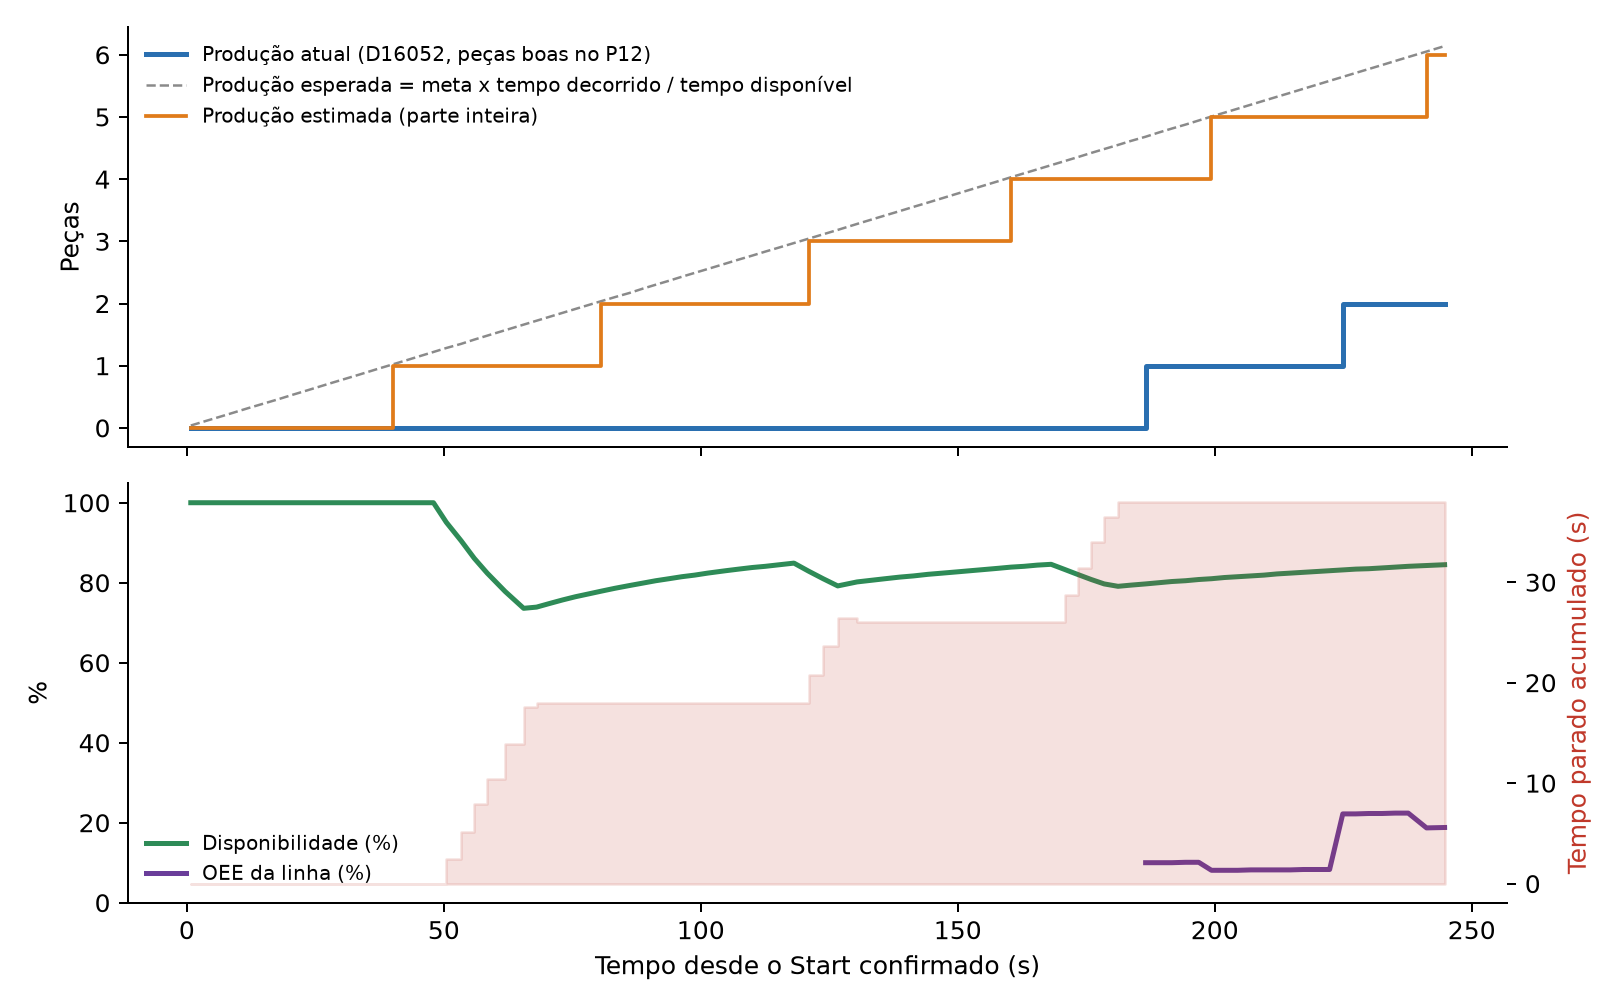
\includegraphics[width=0.95\textwidth]{Imagens/demo_producao_oee.png}
    \caption{Produção atual, esperada e estimada (acima); disponibilidade, OEE e tempo parado acumulado (abaixo), conforme \cod{/api/snapshot}. (arquivo: Imagens/demo\_producao\_oee.png)}
    \label{fig:oee}
\end{figure}

\subsection{Evidência: dados reais do receptor}

O banco do receptor da instalação (\cod{simulador/data/reference\_receiver.db}) contém 127 recepções de eventos (64 ON e 63 OFF, todas do tipo \cod{00 01}) entre 27/09/2026 e 21/11/2026: 18 em 27/09 (os eventos reais do CLP da seção 3.5), 4 em 30/09, 101 em 20/11 e 4 em 21/11. Delas resultaram 64 ocorrências de parada, todas encerradas (23 de Equipamento, 17 de Qualidade, 17 de Processo e 7 de Material), e 17 defeitos registrados pelo Andon de Qualidade. O plano salvo é de 480 peças em 480 min e o último reset confirmado foi em 21/11/2026 00:24 (\cod{runtime\_meta.last\_reset\_at}).
